% DRAFT v0.1 (2026-11-25). AI-assisted draft generated from the project's code and results.
% Before submission: rewrite in your own words (faculty cap: plagiarism + AI content <= 30%),
% read every cited paper, check every number against reports/phase3/, and follow the target venue's template.
\documentclass[conference]{IEEEtran}
\IEEEoverridecommandlockouts

\usepackage[T1]{fontenc}
\usepackage[utf8]{inputenc}
\usepackage{cite}
\usepackage{amsmath,amssymb,amsfonts}
\usepackage{graphicx}
\usepackage{booktabs}
\usepackage{tabularx}
\usepackage{array}
\usepackage{xcolor}
\usepackage[hidelinks]{hyperref}
\usepackage{xurl}

\graphicspath{{figures/}}
\renewcommand{\tabularxcolumn}[1]{>{\raggedright\arraybackslash}m{#1}}
\newcommand{\ind}{\mathbb{1}}

\begin{document}

\title{Forecasting Refined-Fuel Imports and Supply-Shortfall Risk in Landlocked Economies Under Publication Lag}

\author{\IEEEauthorblockN{Imanbek Mashrapov}
\IEEEauthorblockA{Informatics and Engineering Department\\
Ala-Too International University\\
Bishkek, Kyrgyzstan}}

\maketitle

\begin{abstract}
Landlocked economies import refined fuel over few routes from few suppliers, so a supplier's export restriction can become a domestic shortage within weeks. We test whether monthly physical imports, and the probability of a supply shortfall, can be forecast from public customs data using only what was released on each forecast date. On a UN Comtrade panel of 44 gasoline and distillate series from 22 landlocked countries, we compare seasonal and statistical baselines, local and global LightGBM, and two small global neural networks over 43 monthly origins (2023--2026). Every model sees an observation only after its first release, and intervals are conformally calibrated. Four hypotheses, fixed before any model was trained, were tested with Holm correction. Training one model across countries did not improve Kyrgyz forecasts: a per-series LightGBM was best. The neural networks did not beat gradient boosting, in normal or in shock periods. Supplier and shock features gave a 4.5\% pinball gain on high-dependence series that was not significant. However, the probability of a shortfall derived from the forecast distribution ranked risk much better than supplier concentration: precision--recall AUC 0.19 against 0.065 for the Herfindahl--Hirschman index (base rate 0.074), and recall 30\% against 8\% at a 10\% alert budget ($p<0.001$). The raw probabilities overstate risk about twofold. An as-of Platt recalibration removes this bias but gives no Brier skill beyond the base rate, so the signal lies in the ranking. Concentration indices, the usual security-of-supply measure, carried almost no short-run warning signal in this panel.
\end{abstract}

\begin{IEEEkeywords}
petroleum imports, probabilistic forecasting, supply-shortfall risk, landlocked economies, conformal prediction, gradient boosting, publication lag, UN Comtrade, Kyrgyzstan.
\end{IEEEkeywords}

% =====================================================================
\section{Introduction}

Landlocked economies receive refined fuel across at least one neighbouring country, usually by rail or road, and a single supplier can provide almost all of it. Kyrgyzstan is an extreme case: official statements put Russia's share of supply at about 93\% \cite{economist_stocks,kg24_exempt}. Russia restricted gasoline and diesel exports in September 2023 \cite{gta2023}, banned gasoline exports for six months from March 2024 \cite{enerdata2024} and again from October to December 2025 \cite{gta2025}. Supplies under intergovernmental agreements were formally exempt, yet in mid-2026 AI-95 gasoline ran out at Bishkek stations and stocks were reported at two to three weeks against a target of 2.5 months \cite{kwan2026,kunuz2026,economist_stocks}. A formal exemption did not guarantee physical supply.

Two kinds of tools are available to a planner. Security-of-supply indices, such as the Herfindahl--Hirschman index (HHI) of supplier shares, describe structural exposure \cite{cohen2011,lecoq2009,ang2015}, but they look backward and have rarely been tested as predictors. Trade forecasting studies mostly predict annual or value flows for single countries, often with information that was not available on the forecast date \cite{santi2023,pradhan2023,khajoui2024}. The closest precedent, Kwon and Jeong \cite{kwon2026}, predicts import disruptions for Korean products and finds concentration a weak short-run signal, but in a maritime economy, for all goods, and as a ranking rather than a calibrated volume.

This paper asks whether monthly physical imports of refined fuel in landlocked economies, and the probability of a shortfall, can be forecast out of sample with calibrated uncertainty, using only data that was public at the time. Customs data are released two to four months late and are revised, so a forecast made in a given month must look further ahead than the calendar suggests. Four research questions follow, each with a hypothesis fixed before any model was trained:

\begin{description}
\item[RQ1/H1] Does training across countries help? H1: a global model cuts Kyrgyz MASE by at least 5\% against the best local model at $h=3$.
\item[RQ2/H2] Do neural models beat gradient boosting? H2: not overall, but yes in documented shock windows.
\item[RQ3/H3] Do supplier and shock data add value? H3: they cut pinball loss by at least 3\% on high-dependence series.
\item[RQ4/H4] Do forecast-based warnings beat concentration screening? H4: they give higher precision--recall AUC (PR-AUC) and recall at a fixed alert budget than the HHI.
\end{description}

The contributions are: (i) a reproducible route from raw customs records to a validated physical target with release dates, so that every forecast can be replayed as of its origin; (ii) a lag-aware benchmark of statistical, tree-based and neural models on a panel that has not been studied as a group; (iii) the first out-of-sample test, to our knowledge, of supplier concentration as a short-run shortfall signal for single-supplier landlocked importers; and (iv) an open prototype risk monitor. Three of the four hypotheses are not supported, and we report them with the same weight as the one that is.

% =====================================================================
\section{Related Work}\label{sec:related}

\textit{Fuel and trade forecasting.} Country studies of petroleum imports use SARIMA or a single neural model on value data \cite{santi2023,pradhan2023}, and some inflate their samples, for example by interpolating annual data to 200 seasonal points \cite{khajoui2024}. Trade forecasting has moved to graph and neural models at annual or aggregate scale \cite{zhao2026,sellami2024,ma2024}. None of these forecasts monthly physical fuel flows with calibrated uncertainty.

\textit{Security of supply and early warning.} Supply-risk research measures dependence with diversification and risk indices \cite{cohen2011,lecoq2009,ang2015}, or simulates network resilience \cite{chen2025}. Kwon and Jeong \cite{kwon2026} are the only study found that tests such signals out of sample, and found concentration below the base rate as a predictor of disruption onsets.

\textit{Global models and model classes.} Models trained across many series can beat local ones as panels grow \cite{montero2021,semenoglou2021,hewamalage2022}, but the gain depends on how related the series are. Gradient-boosted trees \cite{ke2017,chen2016} dominated the M5 competition \cite{makridakis2022} and still lead on medium-sized tabular data \cite{grinsztajn2022}, while recurrent \cite{hochreiter1997,cho2014,hewamalage2021} and block-stack networks \cite{oreshkin2019} need more data than short economic panels provide.

\textit{Probabilistic evaluation.} Forecasts should maximise sharpness subject to calibration and be scored with proper rules \cite{gneiting2007}. Conformalised quantile regression \cite{romano2019} corrects interval coverage without distributional assumptions, and neural networks are often miscalibrated \cite{guo2017}. Rolling-origin evaluation \cite{tashman2000,bergmeir2018}, scaled errors \cite{hyndman2006} and the Diebold--Mariano test with the Harvey correction \cite{diebold1995,harvey1997} are the accepted standard.

% =====================================================================
\section{Data}\label{sec:data}

\subsection{Source and target}
Monthly bilateral import records were collected from the UN Comtrade API \cite{comtrade} for 43 candidate landlocked economies, with HS six-digit codes from 2015 to August 2026 (snapshot of 2 November 2026; 878 stored responses, each with retrieval date and hash). Two targets are modelled: a gasoline proxy (HS 271011 and 271012) and distillates including blends (HS 271019 and 271020). Six-digit codes cannot separate diesel from jet fuel or fuel oil, so the second target is labelled distillates, not diesel.

Net mass is taken from the net-weight field when positive, otherwise from a quantity field only when its unit is kilograms. A row with a volume must imply a plausible density (0.68--0.80 kg/L for gasoline). Monthly totals are sums of partner rows rather than the aggregate World row, which can be zero while partners report trade. Unit values are checked against product bands and against their Brent-deflated 13-month median; an implausibly low unit value signals overstated mass, which is removed while the record is kept. Missing months are never interpolated or filled with zero.

\subsection{Panel and validation}
Series were assigned to tiers by fixed rules: Tier 1 needs at least 120 observed months, at least 85\% coverage, no gap over six months and data to mid-2025; Tier 2 needs 84 observed months. Tier 1 contains 22 series from 13 countries and is used for evaluation; Tiers 1 and 2 together (44 series, 22 countries) train the global models. Kyrgyzstan is the only Central Asian country in Tier 1. Kyrgyz gasoline mass agrees with the national energy balance \cite{nsc_balance} within a mean absolute 3.7\% from 2018, and partner rows with mass cover at least 90\% of import value in 99.4\% of 6,505 series-months.

\subsection{Release dates}
Each record carries the date it was first released, which we use to decide what was visible at a forecast origin. The median publication lag fell from 180--410 days for 2015--2019 records to 82 days for 2024 and 62 days for 2026, but some reporters publish a year or more late. For older months the release date belongs to the latest revision, so treating it as the first release is conservative: it can hide data that existed earlier, never reveal data early.

\subsection{External data and events}
Brent prices \cite{eia_brent}, the geopolitical risk index and its Russia component \cite{caldara2022}, exchange rates and consumer prices are shifted by their release delays (one month for Brent and the risk indices, two months for exchange rates and consumer prices). A calendar of 37 documented supply events affecting 22 panel countries was coded by hand from public sources (export bans, transit disruptions, foreign-exchange shortages and similar), each with an announcement date and source links. Events enter features only from their announcement and only while known to be active.

% =====================================================================
\section{Methodology}\label{sec:method}

\subsection{As-of information sets and tasks}
A forecast origin $\tau$ is the last day of a month. Observation $y_{it}$ of series $i$ in month $t$ belongs to the information set $\mathcal{F}_{i\tau}$ only if its release date $r_{it}\le\tau$. Each forecast concerns months $\tau+1$, $\tau+3$ and $\tau+6$ and the mean of months $\tau+1$ to $\tau+3$. Because of the lag, a one-month forecast usually lies three to four months beyond the last visible observation. Targets are measured relative to a series level,
\begin{equation}
z_{i,\tau+h}=\log(1+y_{i,\tau+h})-\ell_{i\tau},
\end{equation}
where $\ell_{i\tau}$ is the mean log mass of the last 12 visible months. This makes series of different size comparable in one global model.

Features, all taken from $\mathcal{F}_{i\tau}$, are: 18 calendar lags, the last visible value and the mean of the last three, seasonal lags at 12 and 24 months before the target, data age, volatility and month of year; supplier structure (trailing 12-month HHI, largest-supplier share, Russia's share); external indicators; an as-of unit-value signal; and counts of active and recently announced shock events.

\subsection{Models}
Local benchmarks are the naive forecast, the seasonal naive, the 12-month mean, exponential smoothing with additive seasonality (fitted to the latest unbroken run of at least 36 months), and SARIMA(0,1,1)(0,1,1)$_{12}$ on log mass, whose state-space form handles gaps. ETS and SARIMA quantiles come from 400 simulated paths. Naive-family quantiles come from the same rule's past errors whose targets had been released. Learned models output five quantiles (0.025, 0.1, 0.5, 0.9, 0.975) under the pinball loss: LightGBM \cite{ke2017} fitted per series (local) or across all 44 series with a country identifier (global), a residual multilayer perceptron in the style of a block stack \cite{oreshkin2019}, and a gated recurrent unit \cite{cho2014} over the lag sequence. Both networks have 64 hidden units, an eight-dimensional country embedding and dropout, and are averaged over five seeds. Learned models are refitted every three origins on examples whose targets had been released by the refit date. Hyperparameters are fixed defaults, identical across folds.

\subsection{Conformal calibration}
For each model and task, intervals are adjusted by conformalised quantile regression \cite{romano2019}. At origin $\tau$ the scores $s=\max(\hat q_{\mathrm{lo}}-z,\ z-\hat q_{\mathrm{hi}})$ come from forecasts made at the previous 24 origins whose targets were released by $\tau$, pooled across series. The interval is widened (or narrowed) by the $\lceil (n+1)(1-\alpha)\rceil/n$ empirical quantile of the scores, separately for the 80\% and 95\% intervals.

\subsection{Shortfall target and probability}
Let $Q_{it}$ be the mean import mass over months $t-2$ to $t$ and $B_{it}$ the mean of $Q$ at the same months of the previous three years. A shortfall is
\begin{equation}
S_{it}=\ind\left[Q_{it}/B_{it}<0.75\right].
\end{equation}
Rather than train a classifier on these rare and noisy labels, the probability is read from the forecast distribution of the three-month mean:
\begin{equation}
\hat p_{i,\tau}=\Pr\!\left(Q_{i,\tau+3}<0.75\,B_{i\tau}\mid\mathcal{F}_{i\tau}\right),
\end{equation}
where $B_{i\tau}$ uses only visible data. The predictive distribution function is linear between the conformal quantiles, with normal tails fitted to the outer pair. The HHI benchmark is the trailing 12-month index at the origin. Because the volume labels matched documented events poorly in a separate check (a label fired in 13 of 33 supply events), we also score an event label: the target window overlaps a documented supply-shortfall event, extended by two months.

\subsection{Evaluation protocol}
Origins run monthly from January 2021. Origins in 2021--2022 serve only as calibration history and for choosing between the two networks. The 43 test origins run from January 2023 to July 2026, the last origin with a released target. Point accuracy is measured by MASE \cite{hyndman2006}, scaled by each series' in-sample seasonal difference at the origin. Probabilistic accuracy is measured by the mean pinball loss on the same scale, together with empirical coverage. Model comparisons are made on cases where every model produced a forecast. The HLN-corrected Diebold--Mariano test \cite{diebold1995,harvey1997} is applied to the per-origin mean loss differential, and the four primary $p$-values are adjusted by Holm's method \cite{holm1979}. For H4 the difference in PR-AUC \cite{saito2015} is tested with a moving-block bootstrap over origins (block of six, 2,000 draws), and the Brier score \cite{brier1950} is also reported. Ablations remove one information source at a time from the global LightGBM.

% =====================================================================
\section{Results}\label{sec:results}

\subsection{Point and probabilistic accuracy}
Table~\ref{tab:accuracy} reports accuracy on the Tier 1 series. Global LightGBM has the lowest MASE at one, three months and on the three-month mean, though its lead over the 12-month mean and ETS is small (Fig.~\ref{fig:mase}). Its probabilistic advantage is larger: its pinball loss at $h=3$ is 0.244, against 0.305 for local LightGBM and 0.40--0.47 for ETS and SARIMA. Both neural networks are worse than the 12-month mean on point accuracy. The naive and seasonal naive forecasts are clearly worst, which confirms that the lag-aware setting is hard: the last visible value is several months old.

Before calibration, the learned models' 80\% intervals were too narrow, covering 37--67\% of outcomes (Table~\ref{tab:accuracy}). After the conformal step, every model covers 84--89\% at the 80\% level and 97--99\% at the 95\% level. The intervals now err slightly on the wide side, probably because the calibration scores pool all 44 series, including the noisier Tier 2 series.

\begin{table}[t]
\centering
\caption{Accuracy on Tier 1 series, test origins 2023--2026. MASE by task; pinball loss and 80\% coverage (raw $\rightarrow$ conformal) at $h=3$. Lower MASE and pinball are better.}
\label{tab:accuracy}
\small
\setlength{\tabcolsep}{3pt}
\begin{tabular}{@{}lccccc c@{}}
\toprule
 & \multicolumn{4}{c}{MASE} & & \\
\cmidrule(lr){2-5}
Model & $h{=}1$ & $h{=}3$ & $h{=}6$ & 3-mo & Pinball & Cov.\ 80\%\\
\midrule
Naive & 1.200 & 1.264 & 1.297 & 1.416 & 1.795 & .79$\rightarrow$.84\\
Seasonal naive & 1.136 & 1.137 & 1.148 & 1.075 & 2.460 & .83$\rightarrow$.88\\
12-month mean & 0.947 & 0.989 & 1.036 & 1.006 & 1.313 & .81$\rightarrow$.86\\
ETS & 0.964 & 0.983 & \textbf{0.990} & 1.148 & 0.404 & .86$\rightarrow$.86\\
SARIMA & 1.007 & 1.059 & 1.069 & 1.335 & 0.472 & .89$\rightarrow$.85\\
LightGBM local & 0.974 & 0.982 & 1.011 & 1.009 & 0.305 & .37$\rightarrow$.89\\
LightGBM global & \textbf{0.929} & \textbf{0.976} & 1.015 & \textbf{0.981} & \textbf{0.244} & .67$\rightarrow$.86\\
MLP global & 1.017 & 1.064 & 1.121 & 1.049 & 0.315 & .49$\rightarrow$.86\\
GRU global & 1.032 & 1.092 & 1.154 & 1.072 & 0.335 & .49$\rightarrow$.89\\
\bottomrule
\end{tabular}
\end{table}

\begin{figure}[t]
\centering
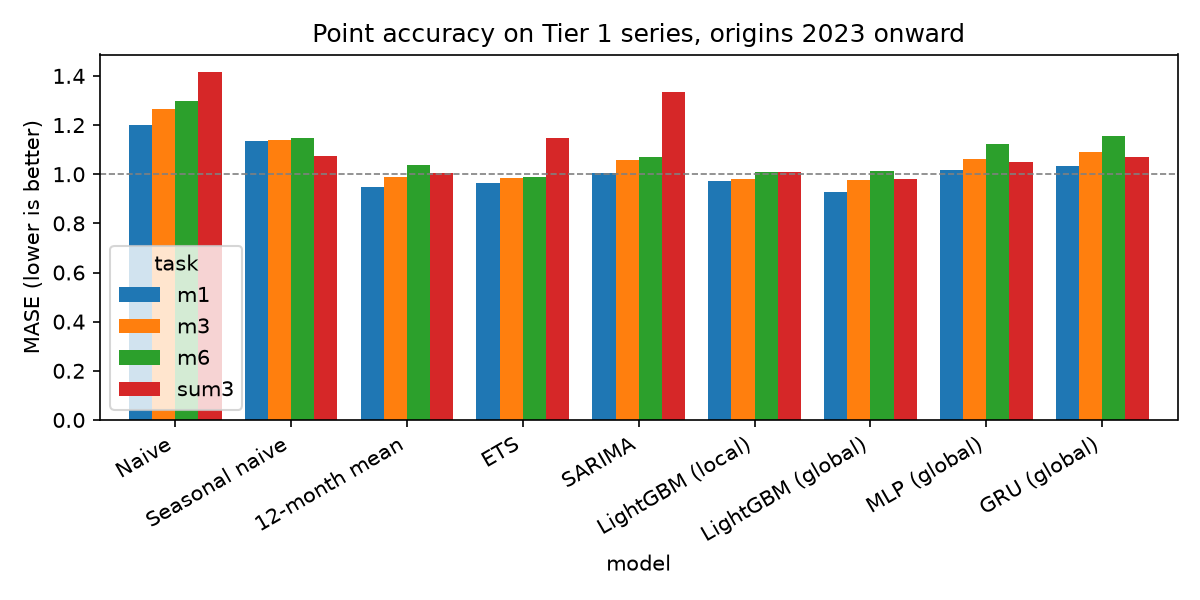
\includegraphics[width=\columnwidth]{fig01_mase_by_model.png}
\caption{MASE by model and task on Tier 1 series. The dashed line marks the historical seasonal-naive error.}
\label{fig:mase}
\end{figure}

\subsection{Hypothesis tests}
Table~\ref{tab:hyp} summarises the four tests.

\textit{H1 (not supported).} For the two Kyrgyz series at $h=3$ the best local model was local LightGBM (MASE 0.875), and global LightGBM was 13.8\% worse (0.996; 95\% CI $-26.0\%$ to $+1.5\%$). Global LightGBM did beat the seasonal naive forecast ($p=0.004$), so pooling is useful against a weak benchmark but not against a well-specified local model. For Kyrgyz gasoline, local LightGBM (0.786) and ETS (0.843) were the two best models.

\textit{H2 (not supported).} The multilayer perceptron, chosen over the GRU on the 2021--2022 calibration origins, was 12.0\% worse than global LightGBM on MASE overall and 12.1\% worse in documented shock windows (111 cases). The pinball gap was larger, 31\% overall and 21\% in shocks. The first half of H2 holds, since the networks did not beat gradient boosting, but the second half fails: the networks had no advantage in shocks.

\textit{H3 (not supported).} On the 17 series whose largest supplier held at least 70\% before 2023, adding supplier, shock, external and unit-value features to an own-history LightGBM cut pinball loss by 4.5\% (95\% CI $-3.0\%$ to $+12.4\%$; $p=0.16$). The point estimate exceeds the 3\% target, but the evidence is not strong enough to support it.

\textit{H4 (supported).} See Section~\ref{sec:warnings}.

\begin{table}[t]
\centering
\caption{Hypothesis tests. Relative change of the first model against the second (positive = better); one-sided HLN or bootstrap $p$-values, Holm-adjusted over the four tests.}
\label{tab:hyp}
\small
\setlength{\tabcolsep}{3pt}
\begin{tabularx}{\columnwidth}{@{}l X c c c@{}}
\toprule
H & Comparison & Effect & $p_{\mathrm{Holm}}$ & Result\\
\midrule
1 & Global vs local LightGBM, Kyrgyz MASE, $h{=}3$ & $-13.8\%$ & 1.00 & No\\
2 & MLP vs LightGBM, MASE in shock windows & $-12.1\%$ & 1.00 & No\\
3 & Full vs own-history LightGBM, pinball, high dependence & $+4.5\%$ & 0.49 & No\\
4 & Shortfall probability vs HHI, PR-AUC & 0.190 vs 0.065 & $<$0.001 & Yes\\
\bottomrule
\end{tabularx}
\end{table}

\subsection{Shortfall warnings}\label{sec:warnings}
Of 861 test cases on Tier 1 series, 64 (7.4\%) were shortfalls. Ranking cases by the forecast probability gave a PR-AUC of 0.190, against 0.065 for the HHI and 0.090 for the largest-supplier share (Table~\ref{tab:h4}, Fig.~\ref{fig:pr}). The HHI scored below the base rate of 0.074, and the largest-supplier share only slightly above it. The bootstrap interval of the PR-AUC difference was 0.058 to 0.271. Flagging the top 10\% of cases caught 30\% of shortfalls with the forecast probability and 8\% with the HHI. The ranking advantage held at thresholds of 0.70 and 0.80, and was largest against the event-calendar label (PR-AUC 0.387 against 0.107, base rate 0.146). It did not reach significance for the narrower supply-side label, which adds a rising unit-value condition and has only 34 positives ($p=0.11$).

\begin{table}[t]
\centering
\caption{Shortfall warnings on Tier 1 series: PR-AUC of the forecast probability and the HHI, and recall at a 10\% alert budget.}
\label{tab:h4}
\small
\setlength{\tabcolsep}{3pt}
\begin{tabular}{@{}lcccccc@{}}
\toprule
Label & Pos. & Base & \multicolumn{2}{c}{PR-AUC} & \multicolumn{2}{c}{Recall}\\
\cmidrule(lr){4-5}\cmidrule(lr){6-7}
 & & & Fcst & HHI & Fcst & HHI\\
\midrule
$Q/B<0.75$ (primary) & 64 & .074 & \textbf{.190} & .065 & \textbf{.30} & .08\\
$Q/B<0.70$ & 45 & .052 & \textbf{.148} & .048 & \textbf{.31} & .09\\
$Q/B<0.80$ & 95 & .110 & \textbf{.234} & .089 & \textbf{.25} & .06\\
Supply-side & 34 & .039 & .098 & .037 & .32 & .06\\
Event calendar & 126 & .146 & \textbf{.387} & .107 & \textbf{.30} & .00\\
\bottomrule
\end{tabular}
\end{table}

\begin{figure}[t]
\centering
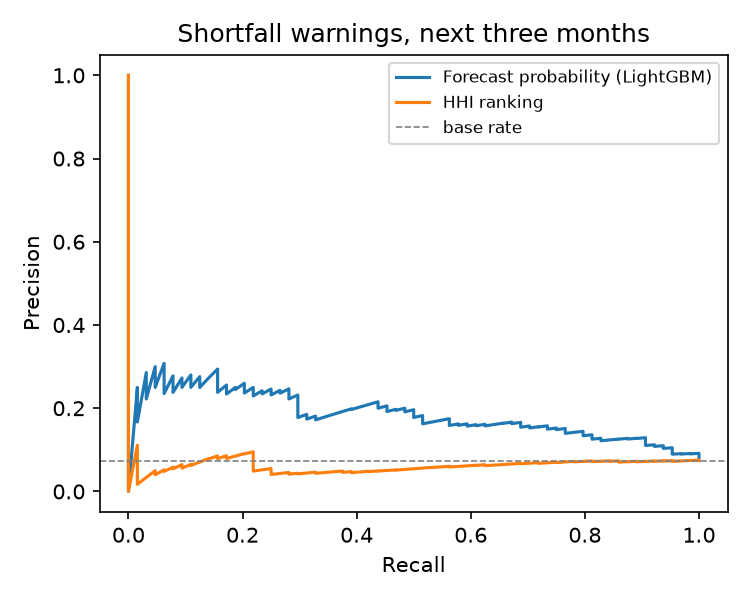
\includegraphics[width=0.85\columnwidth]{fig03_shortfall_pr.png}
\caption{Precision--recall curves for next-three-month shortfalls: forecast probability and HHI ranking.}
\label{fig:pr}
\end{figure}

Ranking and calibration are different properties, however. Fig.~\ref{fig:rel} shows that the probabilities overstate risk throughout: cases given a mean probability of 0.29 had a shortfall frequency of 0.13, and cases given 0.48 had 0.21. The Brier score, 0.081, is slightly worse than the 0.069 of a constant base-rate forecast. A likely reason is that the probability is read from the lower tail of intervals that are, by the coverage results above, somewhat too wide. The probabilities are therefore useful for deciding which series to watch, but not as stated frequencies.

\textit{Recalibration (exploratory).} After seeing this result we added a recalibration step that was not part of the hypotheses. At each origin, a logistic map from $\mathrm{logit}(\hat p)$ to the realised label is fitted on the previous 24 origins whose outcomes had been released, pooled over all 44 series (Platt scaling). A second variant fits the map once, in January 2023, and keeps it fixed. Table~\ref{tab:recal} compares them on the same 861 cases. Both remove most of the overstatement (Fig.~\ref{fig:rel}), and the Brier score falls from 0.081 to 0.070 (rolling) and 0.069 (fixed). Neither is meaningfully better than a constant base-rate forecast: the largest gain over the base-rate Brier, at the 0.80 threshold, is 0.001. The fixed map is monotone, so it keeps the PR-AUC of 0.190. The rolling map keeps the ranking within each month but changes the scale between months, which lowers the pooled PR-AUC to 0.137. The forecast distribution therefore tells us \emph{which} series are at risk, but not reliably \emph{how likely} a shortfall is.

\begin{table}[t]
\centering
\caption{Shortfall probabilities before and after as-of recalibration (exploratory), $Q/B<0.75$, 861 cases, base rate 0.074 (base-rate Brier 0.0688).}
\label{tab:recal}
\small
\begin{tabular}{@{}lcccc@{}}
\toprule
Probability & Mean $\hat p$ & Brier & PR-AUC & Recall@10\%\\
\midrule
Raw & 0.171 & 0.0806 & 0.190 & 0.30\\
Recalibrated, rolling & 0.100 & 0.0697 & 0.137 & 0.22\\
Recalibrated, fixed & 0.140 & 0.0688 & 0.190 & 0.30\\
\bottomrule
\end{tabular}
\end{table}

\begin{figure}[t]
\centering
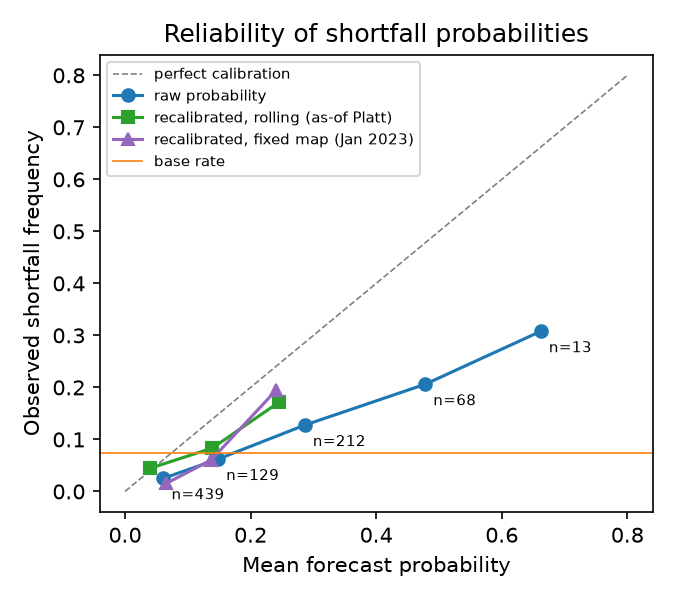
\includegraphics[width=0.8\columnwidth]{fig06_shortfall_reliability.png}
\caption{Reliability of shortfall probabilities, raw and after as-of recalibration. Points below the diagonal mean that risk is overstated. Recalibrated bins with fewer than 10 cases are omitted.}
\label{fig:rel}
\end{figure}

\subsection{Ablation}
Table~\ref{tab:abl} removes one component at a time from global LightGBM at $h=3$. No single information source made a large difference to the median forecast; their value showed in the quantiles. Removing external indicators or reducing the model to its own history raised the pinball loss by 3.6--3.7\%, and removing shock features raised it by 2.7\%. Removing supplier features changed little. Training on strict importers only raised the pinball loss on those importers by 16.5\%, which suggests that the producers and refiners in the panel help the model learn the shape of uncertainty. Local training (one LightGBM per series) raised it by 24.9\%. Leaving Kyrgyzstan out of training hurt Kyrgyz forecasts only slightly (pinball $+3.8\%$), which agrees with the H1 finding that pooled data add little specific to this country. A model frozen at December 2021 and never refitted was slightly better than the refitted one ($-2.4\%$ pinball), so refitting every quarter brought no gain in this window. Without the conformal step the median is unchanged, and the pinball loss is 9.1\% lower, but the 80\% coverage falls to 0.68.

\begin{table}[t]
\centering
\caption{Ablation of global LightGBM at $h=3$ (Tier 1). Change against the full model; positive = worse.}
\label{tab:abl}
\small
\setlength{\tabcolsep}{4pt}
\begin{tabular}{@{}lrrc@{}}
\toprule
Variant & MASE & Pinball & Cov.\ 80\%\\
\midrule
Own history only & $-3.1\%$ & $+3.7\%$ & .89\\
No external indicators & $-1.4\%$ & $+3.6\%$ & .88\\
No shock features & $+1.1\%$ & $+2.7\%$ & .87\\
No unit-value signal & $-0.3\%$ & $+1.9\%$ & .86\\
No supplier features & $-2.4\%$ & $-0.1\%$ & .86\\
Strict importers only$^a$ & $-0.3\%$ & $+16.5\%$ & .94\\
Local training & $+0.8\%$ & $+24.9\%$ & .89\\
Training data from 2018 & $-0.1\%$ & $+0.3\%$ & .88\\
Frozen at Dec 2021 & $-2.6\%$ & $-2.4\%$ & .88\\
Kyrgyzstan left out$^b$ & $+2.2\%$ & $+3.8\%$ & .74\\
No conformal step & $0.0\%$ & $-9.1\%$ & .68\\
\bottomrule
\multicolumn{4}{@{}l}{\footnotesize $^a$Scored on strict importers. $^b$Scored on Kyrgyz series.}
\end{tabular}
\end{table}

\subsection{Kyrgyzstan}
Fig.~\ref{fig:kgz} shows the three-month-ahead forecasts for Kyrgyzstan. The gasoline intervals widen in 2024--2025, when the Russian export bans increased volatility, and the median does not follow the sharp single-month drops, for example September 2025 (7.9~kt). At the latest origin, October 2026, Kyrgyz gasoline has the second-highest shortfall risk in the panel for the next three months: a raw probability of 0.62, or 0.31 after rolling recalibration. Given the results above, the rank is the informative part.

\begin{figure}[t]
\centering
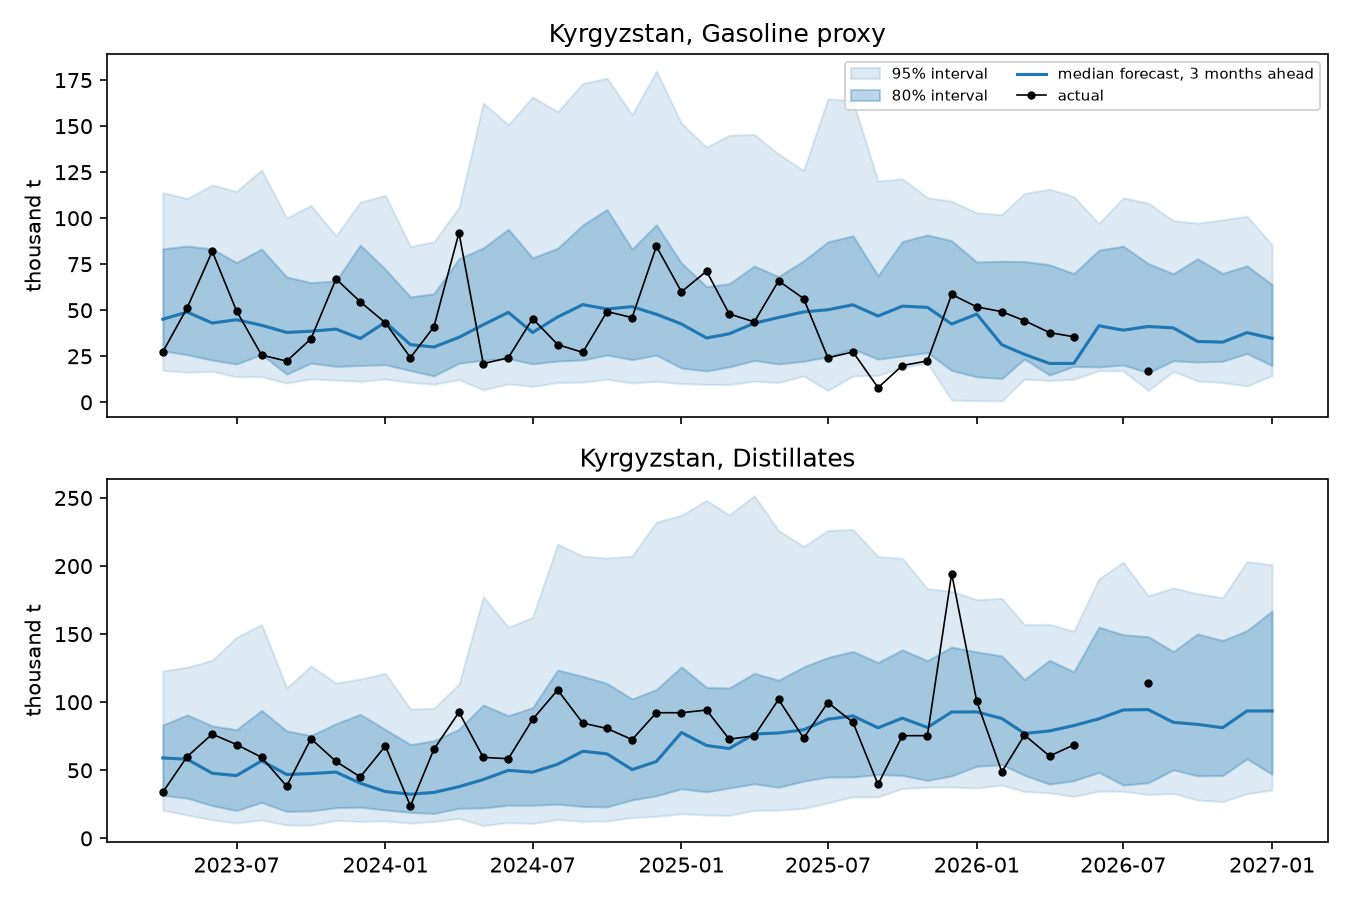
\includegraphics[width=\columnwidth]{fig04_kgz_forecasts.png}
\caption{Kyrgyzstan: actual monthly imports and global LightGBM forecasts made three months earlier, with conformal 80\% and 95\% intervals.}
\label{fig:kgz}
\end{figure}

% =====================================================================
\section{Discussion}\label{sec:discussion}

\textit{Concentration is not a warning signal.} The clearest result is negative for the standard tool. In a panel where many importers rely on one supplier, the HHI and the largest-supplier share ranked future shortfalls no better than chance. This extends Kwon and Jeong's finding for Korea \cite{kwon2026} to single-supplier landlocked importers. Concentration describes exposure, which changes slowly; a shortfall is a short-run event that a volume forecast can see in recent dynamics and seasonal position. The two measures answer different questions, and planners should not use the first to answer the second.

\textit{Pooling and deep learning.} Global training helped the tree model's quantiles across the panel, but not Kyrgyz point accuracy. With 22 heterogeneous countries, a model that fits the average may lose to one that fits the series, which is consistent with simulation evidence that pooling gains reverse as series diverge \cite{montero2021,hewamalage2022}. The networks lost to LightGBM in every window. With about 5,500 training observations this is the expected result \cite{grinsztajn2022}, and we found no sign that shocks favour neural models.

\textit{What a planner can use.} Under realistic publication lags, the forecasts beat simple rules but only modestly on point accuracy. The practical value lies in two places: calibrated intervals for stock planning, and a ranking of which series are most at risk next quarter. Recalibration makes the probability level honest but adds nothing beyond the base rate. Decisions with explicit costs should therefore use the ranking with an alert budget rather than a probability threshold.

% =====================================================================
\section{Limitations and Threats to Validity}\label{sec:limits}

\textit{Data vintage.} One Comtrade snapshot was used. Values for older months are the latest revision, and records from 2025 onward appear to be first releases. Revisions could not be measured; a second snapshot is planned.

\textit{Labels.} Volume-based shortfall labels are a weak proxy for supply stress, as the event check showed. The event-calendar label is built from English-language and official sources, and is thinner for small markets.

\textit{Scope of models.} Random forest, XGBoost, temporal convolutional networks, the full N-BEATS and the Temporal Fusion Transformer were planned but not run. Hyperparameters were not tuned. A tuned or larger network might perform differently, though the data size argues against large gains.

\textit{Statistical power.} With 43 origins and few shock months, pairwise tests have low power; we report effect sizes and intervals alongside $p$-values.

\textit{Post-hoc analysis.} The recalibration step was added after the test results were seen. It is reported as exploratory, and the pre-specified H4 test uses the raw probability.

\textit{Rules.} The cleaning rules and tier thresholds are judgement calls. They were frozen before modelling and recorded with their reasons, but other reasonable choices exist.

% =====================================================================
\section{Conclusion}\label{sec:conclusion}

Public customs data, used strictly as released, support useful but modest forecasts of monthly fuel imports in landlocked economies. They also support a shortfall ranking that is far more informative than supplier concentration. Cross-country pooling and small neural networks did not deliver the gains often assumed, and a well-specified local model remained best for Kyrgyzstan. Recalibrating the shortfall probabilities removes their bias but does not give them skill in level. Future work will look for features that sharpen the lower tail, measure data revisions across snapshots, and extend the event calendar with non-English sources. The code, frozen rules and a prototype monitor are available for replication.

\section*{Data and Code Availability}
All data are public and aggregate. The pipeline, configuration, decision log and evaluation code are in the project repository [URL to be added]; every table and figure is regenerated by \texttt{run.py evaluate}.

\section*{Use of AI Tools}
% Required by the faculty guideline: state tools, purposes, substantial generated elements and how output was checked.
[To be completed by the author: tools used, for which parts of the code and text, and how the output was reviewed and validated.]

\section*{Acknowledgment}
The author thanks the supervisor, Dr.\ Remudin Mekuria, for guidance.

\bibliographystyle{IEEEtran}
\bibliography{references}

\end{document}
